\section{Task-Conditioned Disagreement Analysis}
\label{sec:task-conditioned-disagreement}

The main paper analyzes how teacher--verifier disagreement changes with prompt
length in two representative tasks. Here, we complement that analysis with a
task-conditioned view of four GoLongRL task families containing at least 500
prompts. For Multi-Table Extraction and High-Recall Retrieval, we aggregate the
same frozen responses used in Figure~1 over prompts shorter than 32K, without
separating the two length ranges. Each of the other task rows is likewise
computed from eight fixed Qwen3-8B responses per prompt. Overall pools all nine
task families by giving each informative prompt equal weight.

Within each informative rollout group, the pairwise disagreement rate is the
fraction of response pairs with distinct verifier rewards for which the OPD and
verifier orderings disagree. We average this rate across prompts. The top-1
mismatch rate is the fraction of these groups in which the response with the
highest trajectory-level OPD score does not attain the group's highest verifier
reward.
Their variation across task families complements the length-conditioned trends
in the main paper and motivates comparing the two assessments locally within
each rollout group. Because the responses are fixed, the analysis characterizes
signal disagreement rather than task-specific training gains or causal effects
of task type or context length.

\begin{figure}[H]
\centering
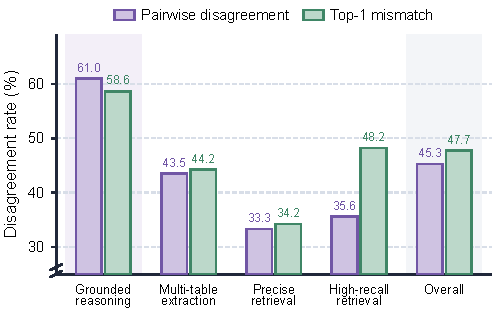
\includegraphics[width=0.74\columnwidth]{Figures/gcopd_diagnostics/gcopd_task_conditioned_disagreement.pdf}
\caption{Task-conditioned teacher--verifier disagreement in four GoLongRL task
families. Bars report prompt-macro pairwise disagreement rates and top-1
mismatch rates over rollout groups with at least two distinct verifier rewards.
Overall pools all nine task families.}
\label{fig:task-conditioned-mismatch}
\end{figure}

\FloatBarrier
\section{GC-OPD Implementation Details}

Using the notation of the main paper, $A^{(i)}_t$ is the detached token-level OPD
advantage, $s^{(i)}=(T^{(i)})^{-1}\sum_t A^{(i)}_t$ is its trajectory-level OPD score, and
$R^{(i)}$ is the verifier reward. The main paper defines the compact
pre-clipping update $A'^{(i)}_t$. Here, $T^{(i)}$ is the number of valid tokens
in response $i$, $G$ is the rollout-group size, and $\beta$ is the residual
coefficient in the main update. This section specifies the numerical guards and
update order used in the completed runs. The thresholds $\tau_G$ and $\tau_T$
guard group-level and token-level standard deviations, respectively, and
$a_{\max}$ is the final advantage-clipping bound. For $h\in\{R,s\}$, let
$\mu_h$ and $\sigma_h$ denote the population mean and standard deviation over
the $G$ responses. The implemented residual is
\begin{equation}
\rho^{(i)}=
\begin{cases}
\frac{R^{(i)}-\mu_R}{\sigma_R}
-\frac{s^{(i)}-\mu_s}{\sigma_s},
&\sigma_R,\sigma_s>\tau_G,\\
0,&\text{otherwise}.
\end{cases}
\label{eq:guarded-residual}
\end{equation}
If either group-level signal has negligible variation, the residual is zero
and the update reduces to vanilla OPD.

The token credit uses an analogous guard. Within response $i$, let
$\sigma_A^{(i)}$ denote the population standard deviation of its valid token
advantages. The guarded RACA credit is
\begin{align}
u^{(i)}_t&=
\begin{cases}
\dfrac{A^{(i)}_t-s^{(i)}}{\sigma_A^{(i)}},
&T^{(i)}\geq2\ \text{and}\ \sigma_A^{(i)}>\tau_T,\\
0,&\text{otherwise},
\end{cases}
\label{eq:normalized-token-advantage}\\
c^{(i)}_t&=1+\tanh\!\left(\frac{u^{(i)}_t}{2}\right),
\label{eq:implemented-token-credit}
\end{align}
Here, $u^{(i)}_t$ is the token's OPD advantage relative to the response mean,
measured in units of the within-response standard deviation. It describes
relative OPD support rather than token correctness. Thus negligible token
variation gives unit credit. After forming
$A'^{(i)}_t$, we clip it to $[-a_{\max},a_{\max}]$ before the policy update.
Table~\ref{tab:training} reports $\tau_G$, $\tau_T$, and $a_{\max}$. These
Given the OPD advantages and verifier rewards, these operations require no
additional teacher or student forward pass.

\begin{algorithm}[H]
\caption{Group-Calibrated On-Policy Distillation}
\label{alg:gcopd}
\begin{algorithmic}[1]
\REQUIRE Prompt batch $\mathcal{B}$; trainable student policy $\pi_\theta$; teacher $\pi_T$;
verifier $V$; group size $G$; residual coefficient $\beta$; thresholds
$\tau_G,\tau_T$; clipping bound $a_{\max}$
\ENSURE Updated student policy $\pi_\theta$
\STATE Set $\theta_{\mathrm{old}}\leftarrow\theta$ and freeze
$\pi_{\theta_{\mathrm{old}}}$ for rollout generation
\FOR{each prompt $\mathbf{x}\in\mathcal{B}$}
  \STATE Sample $\mathcal{G}(\mathbf{x})=\{\mathbf{y}^{(i)}\}_{i=1}^{G}$
  from $\pi_{\theta_{\mathrm{old}}}(\cdot\mid\mathbf{x})$
  \FOR{$i=1,\ldots,G$}
    \STATE $R^{(i)}\leftarrow V(\mathbf{x},\mathbf{y}^{(i)})$
    \STATE Compute detached $A^{(i)}_t$ under $\pi_T$ and
    $\pi_{\theta_{\mathrm{old}}}$ for
    $t=1,\ldots,T^{(i)}$
    \STATE $s^{(i)}\leftarrow (T^{(i)})^{-1}
    \sum_{t=1}^{T^{(i)}} A^{(i)}_t$
  \ENDFOR
  \STATE Compute population statistics $(\mu_R,\sigma_R)$ and
  $(\mu_s,\sigma_s)$ over the $G$ responses
  \IF{$\sigma_R>\tau_G \land \sigma_s>\tau_G$}
    \STATE $\rho^{(i)}\leftarrow
    \dfrac{R^{(i)}-\mu_R}{\sigma_R}
    -\dfrac{s^{(i)}-\mu_s}{\sigma_s}$ for $i=1,\ldots,G$
  \ELSE
    \STATE $\rho^{(i)}\leftarrow0$ for all $i$
  \ENDIF
  \FOR{each response $i$}
    \STATE Compute $\sigma_A^{(i)}$ from
    $\{A^{(i)}_t\}_{t=1}^{T^{(i)}}$
    \IF{$T^{(i)}\geq2 \land \sigma_A^{(i)}>\tau_T$}
      \STATE $u^{(i)}_t\leftarrow
      \dfrac{A^{(i)}_t-s^{(i)}}{\sigma_A^{(i)}}$
      for $t=1,\ldots,T^{(i)}$
      \STATE $c^{(i)}_t\leftarrow
      1+\tanh\!\left(u^{(i)}_t/2\right)$
      for $t=1,\ldots,T^{(i)}$
    \ELSE
      \STATE $u^{(i)}_t\leftarrow0$ and $c^{(i)}_t\leftarrow1$ for
      $t=1,\ldots,T^{(i)}$
    \ENDIF
    \STATE $A'^{(i)}_t\leftarrow A^{(i)}_t+
    \beta c^{(i)}_t\rho^{(i)}$ for $t=1,\ldots,T^{(i)}$
    \STATE $\widehat A^{(i)}_t\leftarrow
    \operatorname{clip}(A'^{(i)}_t,-a_{\max},a_{\max})$ for all $t$
  \ENDFOR
\ENDFOR
\STATE Update $\pi_\theta$ using the same policy surrogate as vanilla OPD, with
$\widehat A^{(i)}_t$ as the token-level advantages
\end{algorithmic}
\end{algorithm}

\section{Experimental Details}

\subsection{Models, Data, and Training Configuration}

We initialize Qwen3-4B and Qwen3-8B students from their official checkpoints
and use Qwen3-30B-A3B-Thinking-2507 as the teacher. Students generate in
no-thinking mode, and the teacher scores the sampled response tokens without
generating separate responses.

The 32K-filtered GoLongRL training file contains 9,527 prompts.
Table~\ref{tab:data} reports its prompt-length distribution, complementing the
task-family and verifier statistics in the main paper. The median, 90th
percentile, and maximum lengths are 9,923, 26,940, and 32,766 tokens.

\begin{table}[t]
\captionsetup{justification=raggedright,singlelinecheck=false,skip=6pt}
\caption{Prompt-length distribution of the exact 32K-filtered training file.}
\label{tab:data}
\centering
{\small
\setlength{\tabcolsep}{6pt}
\renewcommand{\arraystretch}{1.05}
\begin{tabular*}{0.36\textwidth}{@{\extracolsep{\fill}}cc@{}}
\toprule
\textbf{Prompt length} & \textbf{Samples} \\
\midrule
$\leq 2$K & 2,222 \\
2--8K & 1,958 \\
8--16K & 2,155 \\
16--24K & 1,914 \\
24--32K & 1,278 \\
\midrule
Total & 9,527 \\
\bottomrule
\end{tabular*}
}
\end{table}

Table~\ref{tab:training} records the common configuration. Raw rows receive no
training; every trained method uses this configuration and is evaluated at
its final checkpoint.

\begin{table}[t]
\captionsetup{justification=raggedright,singlelinecheck=false,skip=6pt}
\caption{Shared training configuration and GC-OPD settings.}
\label{tab:training}
\centering
{\small
\setlength{\tabcolsep}{4.0pt}
\renewcommand{\arraystretch}{1.05}
\ifdefined\GCOPDSingleColumnLayout
\begin{tabular}{@{}p{0.38\textwidth}>{\centering\arraybackslash}p{0.35\textwidth}@{}}
\else
\begin{tabular}{@{}p{0.45\columnwidth}>{\centering\arraybackslash}p{0.51\columnwidth}@{}}
\fi
\toprule
\textbf{Setting} & \textbf{Value} \\
\midrule
Training horizon & 100 steps \\
Prompt batch size & 32 \\
Responses per prompt & 8 \\
Maximum prompt length & 32,768 \\
Training response cap & 10,240 \\
Learning rate & $10^{-6}$ \\
Warmup & 0 \\
Weight decay & 0.01 \\
Policy mini-batch size & 4 \\
PPO epochs & 1 \\
PPO clip ratio & 0.2 \\
Loss aggregation & Token mean \\
Rollout temperature & 1 \\
Rollout top-$p$ & 1 \\
Precision & bfloat16 \\
Random seed & 42 \\
Residual coefficient & $\beta=0.10$ \\
Group std. threshold & $\tau_G=10^{-6}$ \\
Token std. threshold & $\tau_T=10^{-6}$ \\
Final advantage clip & $[-10,10]$ ($a_{\max}=10$) \\
\bottomrule
\end{tabular}
}
\end{table}

\paragraph{Compute resources.}
Each training run used eight 80-GB NVIDIA H800 or H100 GPUs. Rollout tensor
parallelism and actor/reference sequence parallelism were both set to 8.

\subsection{Ablation Configurations}
\label{sec:ablation-configurations}

The ablations in the main paper use independent Qwen3-8B training runs under
the shared configuration in Table~\ref{tab:training}. All runs use the same
student initialization, teacher, filtered training data, optimizer, rollout
budget, and 100-step training horizon. They are evaluated at step 100 with the
same five-benchmark pipeline as the main comparison.

\paragraph{Added-signal ablation.}
Vanilla OPD provides the common anchor for this comparison. The three augmented
variants use the same RACA credit and a scalar coefficient of 0.10, while
changing the signal added to the vanilla OPD advantage. Their updates before
final advantage clipping are
\begin{align}
A'^{(i)}_t&=A^{(i)}_t
&&\text{(vanilla OPD)},\\
A'^{(i)}_t&=A^{(i)}_t+\beta c^{(i)}_tA^{(i)}_t,
\quad \beta=0.10
&&\text{(Additional OPD)},\\
A'^{(i)}_t&=A^{(i)}_t+\beta c^{(i)}_t\tilde{R}^{(i)},
\quad \beta=0.10
&&\text{(Direct reward)},\\
A'^{(i)}_t&=A^{(i)}_t+\beta c^{(i)}_t\rho^{(i)},
\quad \beta=0.10
&&\text{(GC-OPD)}.
\end{align}
The comparison holds the original OPD signal, RACA allocation, and coefficient
fixed. Additional OPD adds another credit-modulated OPD term, Direct reward uses the group-normalized verifier reward
$\tilde{R}^{(i)}$, whereas GC-OPD subtracts the group-normalized trajectory
OPD score and uses $\rho^{(i)}=\tilde{R}^{(i)}-\tilde{s}^{(i)}$. It
therefore separates the effect of adding another OPD-derived term from adding verifier feedback, and tests whether accounting for the relative preference already expressed by OPD improves upon adding verifier feedback directly.

\paragraph{Token-allocation ablation.}
This comparison fixes the signed residual and the same $\beta=0.10$ used by
the main configuration, so every calibrated variant uses
$A'^{(i)}_t=A^{(i)}_t+0.10c^{(i)}_t\rho^{(i)}$. Only the token credit
$c^{(i)}_t$ changes. Uniform allocation sets
$c^{(i)}_t=1$. Absolute OPD is a token-allocation control, not an alternative
trajectory-level signal. It assigns credit in proportion to the magnitude of
the tokenwise OPD advantage:
\begin{equation}
c^{(i)}_t=\operatorname{clip}_{[0,5]}\!\left(
\frac{\lvert A^{(i)}_t\rvert}
{(T^{(i)})^{-1}\sum_{v=1}^{T^{(i)}}\lvert A^{(i)}_v\rvert}
\right),
\label{eq:absolute-opd-credit}
\end{equation}
The upper bound of 5 limits extreme token weights, and unit credit is used when
the denominator is numerically negligible. RACA uses
Equation~\ref{eq:implemented-token-credit}. Thus this comparison holds the
trajectory-level residual and its coefficient fixed while isolating how the
correction is distributed across response tokens.

\subsection{Baselines under the Shared Setup}

All trained baselines share the student initialization, teacher, filtered
training data, rollout budget, optimizer, training horizon, and clipped
surrogate. We hold these factors fixed to isolate each method's principal
training-signal mechanism. The comparisons should therefore be interpreted as
controlled mechanism comparisons under a shared setup rather than exact
reproductions of the original experimental recipes. Each method generates its
own trajectories on-policy. Let
$p_{T,t}$, $p_{S,t}$, and $p_{0,t}$ denote the teacher, current-student, and
frozen student-base probabilities of the sampled token. The paragraphs below
record only method-specific implementation choices. To avoid clutter, the
response index $i$ is suppressed in baseline-specific token formulas unless
it is needed explicitly.

\paragraph{Raw checkpoint.}
Raw evaluates the official Qwen3-4B or Qwen3-8B checkpoint without additional
training, using the same downstream evaluation pipeline.

\paragraph{OPD.}
OPD uses $A_t^{\mathrm{OPD}}=\log p_{T,t}-\log p_{S,t}$ as the detached token
advantage. The native verifier is executed by the shared pipeline, but its
terminal score is not added to this advantage. Equivalently, vanilla OPD is
recovered from GC-OPD by setting $\beta=0$, and we use this convention
throughout the supplement.

\paragraph{ExOPD.}
ExOPD replaces the teacher log-probability target with an extrapolated target
anchored at the corresponding frozen student-base checkpoint:
\begin{equation}
A_t^{\mathrm{Ex}}=
\lambda\log p_{T,t}+(1-\lambda)\log p_{0,t}-\log p_{S,t}.
\label{eq:exopd}
\end{equation}
Our runs use $\lambda=1.25$ and the corresponding frozen Qwen3 initialization
as $p_0$, following the default student-base-reference formulation. The
reference contributes only to the detached token target and is not used as a
KL regularizer. In the ExOPD paper, ``reward correction'' denotes the optional
replacement of $p_0$ with the teacher's pre-RL base model. This reference-based
variant is distinct from the verifier reward used by GC-OPD and is not used
here.

\paragraph{Uni-OPD.}
Uni-OPD combines token-level teacher supervision with response-level outcome
separation. Within the eight responses for one prompt, responses with positive
verifier reward form the correct set and the others form the
incorrect set. Let $\bar{s}^{+}$ and $\bar{s}^{-}$ be the mean response-level
OPD scores of these two sets. If both sets exist, the required shift is
\begin{equation}
d=\max\{0,\,\delta-(\bar{s}^{+}-\bar{s}^{-})\}.
\label{eq:uni-margin}
\end{equation}
With bidirectional calibration, $d/2$ is added to every token of a correct
response and subtracted from every token of an incorrect response. Groups
lacking either set receive no margin shift.

For a controlled comparison, we isolate Uni-OPD's outcome-guided margin
calibration and omit its offline and online data-balancing components. This
keeps the training data and rollout budget consistent across methods. The
implementation uses group scope, mean statistics, $\delta=0.4$, and
bidirectional shifts. Following the released implementation, the resulting
group-level shift is added to the original tokenwise OPD advantages. We also
retain the released configuration's teacher--student log-probability-gap mask
with a threshold of 10 as a training-stability setting.

\paragraph{PowerOPD.}
PowerOPD changes the geometry of the token signal from a log-probability gap to
a bounded probability-power difference:
\begin{equation}
A_t^{\mathrm{Power}}=
\operatorname{sg}\!\left[p_{T,t}^{\alpha}-p_{S,t}^{\alpha}\right],
\qquad \alpha=100,
\label{eq:poweropd}
\end{equation}
where $\operatorname{sg}$ denotes stop-gradient. We use this bounded signal as
the method-specific token advantage within the shared clipped surrogate. Both
model scales use $\alpha=100$.

\paragraph{FiRe-OPD.}
Following the released implementation, FiRe-OPD computes the length-normalized
teacher score $q^{(i)}=(T^{(i)})^{-1}\sum_t\log p_{T,t}^{(i)}$ for each
trajectory and applies the actor-micro-batch percentile filter. Token weights
use teacher confidence and student confusion,
\begin{equation}
c_{T,t}=1-\frac{H_{T,t}}{\max H_T},\qquad
c_{S,t}=\frac{H_{S,t}}{\max H_S},
\end{equation}
clipped to $[0,1]$. The OPD advantage is multiplied by
$w_t=(1+\alpha_F c_{T,t})(1+\beta_F c_{S,t})$ after normalizing $w$ to mean one
over valid tokens. Filtered trajectories contribute no policy loss.

Both runs use a 20th-percentile trajectory cutoff and
$\alpha_F=\beta_F=1$. The percentile, entropy maxima, and weight normalization
are recomputed within each actor micro-batch supplied to the loss. The actor
starts from four-response policy mini-batches and may split them further under
dynamic token budgeting.

\subsection{Evaluation Implementation}

Table~\ref{tab:evaluation} records the evaluation units and aggregation rules.
The paragraphs below specify the per-example scorers.

\begin{center}
\begin{minipage}{\columnwidth}
\centering
\captionof{table}{Evaluation units and aggregation for the five reported
long-context benchmark columns.}
\label{tab:evaluation}
{\small
\setlength{\tabcolsep}{2.5pt}
\begin{tabular}{>{\raggedright\arraybackslash}p{0.18\columnwidth}
                >{\raggedright\arraybackslash}p{0.34\columnwidth}
                >{\raggedright\arraybackslash}p{0.38\columnwidth}}
\toprule
Benchmark & Evaluation units & Reported aggregation \\
\midrule
DocMath & Four splits: 200/100/200/300
        & Per-item max(rule, judge); four-split aggregate \\
FRAMES & 824 questions
       & Mean max(CEM, judge) accuracy \\
MRCR & 0--128K $\times$ \{2, 4, 8\} needles
     & Mean prefix-gated sequence ratio \\
CorpusQA & 0--128K $\times$ four domains
         & Overall example accuracy \\
LBv1QA & Five subsets $\times$ 200
       & Macro mean of five subset accuracies \\
\bottomrule
\end{tabular}
}
\end{minipage}
\end{center}

\paragraph{DocMath.}
The evaluator extracts the final answer and applies both the rule-based
numerical/equation checker and a semantic-equivalence judge. The per-example
score is the maximum of these binary decisions. Scores are then aggregated
over the four simple/complex and short/long splits shown in
Table~\ref{tab:evaluation}.

\paragraph{FRAMES.}
After removing any hidden reasoning segment, the scorer applies cover exact
match (CEM). CEM lowercases text, removes punctuation and articles, normalizes
comma-separated numbers, and requires the target as a word-bounded span in the
answer. A sample is correct if either CEM or the semantic-equivalence judge
accepts it.

\paragraph{MRCR.}
Every gold response begins with a sample-specific random prefix. A prediction
without the exact prefix receives zero. Otherwise, the scorer removes the
prefix and computes Python character-level \texttt{SequenceMatcher} similarity
between the prediction and reference. The aggregate includes the 2-, 4-, and
8-needle variants across context lengths.

\paragraph{CorpusQA.}
We use the 0--128K file covering Chinese finance, English finance, English
education, and English real estate. The evaluator extracts text following the
prescribed answer marker when present, then obtains a binary
semantic-equivalence judgment against the generated reference. The reported
column is overall example accuracy across the four domains.

\paragraph{LongBench v1 QA.}
The evaluator extracts the final occurrence of ``Therefore, the answer is''
and falls back to the last non-empty line when the marker is absent. It compares
the extracted answer with every accepted reference and takes the maximum binary
semantic judgment. The reported score is the macro mean over NarrativeQA,
Qasper, HotpotQA, 2WikiMultihopQA, and MuSiQue.

Student serving accepts at most 120,000 input tokens and uses a 131,072-token
model length with YaRN factor 4 and target length 131,072. The completed
evaluation runs cap generation at 8,192 tokens. Inputs that exceed the serving
budget are middle truncated so that both the beginning and end are retained.
Students remain in no-thinking mode, and no method receives a method-specific
evaluation prompt or decoding override. Semantic judging uses
Qwen3-30B-A3B-Instruct-2507 with a 32,768-token context and a 2,048-token
output cap. The reported aggregate is the naive average of the five benchmark
scores.

\section{Auditable Long-Context Case Study}

To make the GC-OPD signal computation concrete, we present one example from
GoLongRL. Its Qwen3-8B no-thinking prompt contains 17,265 tokens and asks which
matrix receives the largest relative improvement from parallel NUMA
optimization: A \texttt{rajat31}, B \texttt{HV15R}, C \texttt{cage15}, or D
\texttt{ldoor}. The dataset's native label is B. The contextual observations
reproduced in Figure~\ref{fig:case} support this label, but do not by themselves
constitute a direct speedup measurement.

This case is an illustrative audit of the signal computation rather than
additional quantitative evidence. We independently reroll the example using
the official Qwen3-8B base checkpoint and Qwen3-30B-A3B-Thinking-2507 as the
teacher. We sample eight responses with temperature 1, top-$p=1$, top-$k=-1$,
seed 42, and a 10,240-token response cap.
Table~\ref{tab:case-tokens} reports representative token signals recomputed
offline with $\beta=0.10$ and $a_{\max}=10$. In the table, the response index
is suppressed within each response block, and
$\Delta A_t=\beta c_t\rho$ denotes the additive residual correction before
clipping.

\ifdefined\GCOPDSingleColumnLayout
\begin{figure}[t]
\else
\begin{figure*}[!t]
\fi
\centering
\ifdefined\GCOPDSingleColumnLayout
\makebox[\textwidth][c]{%
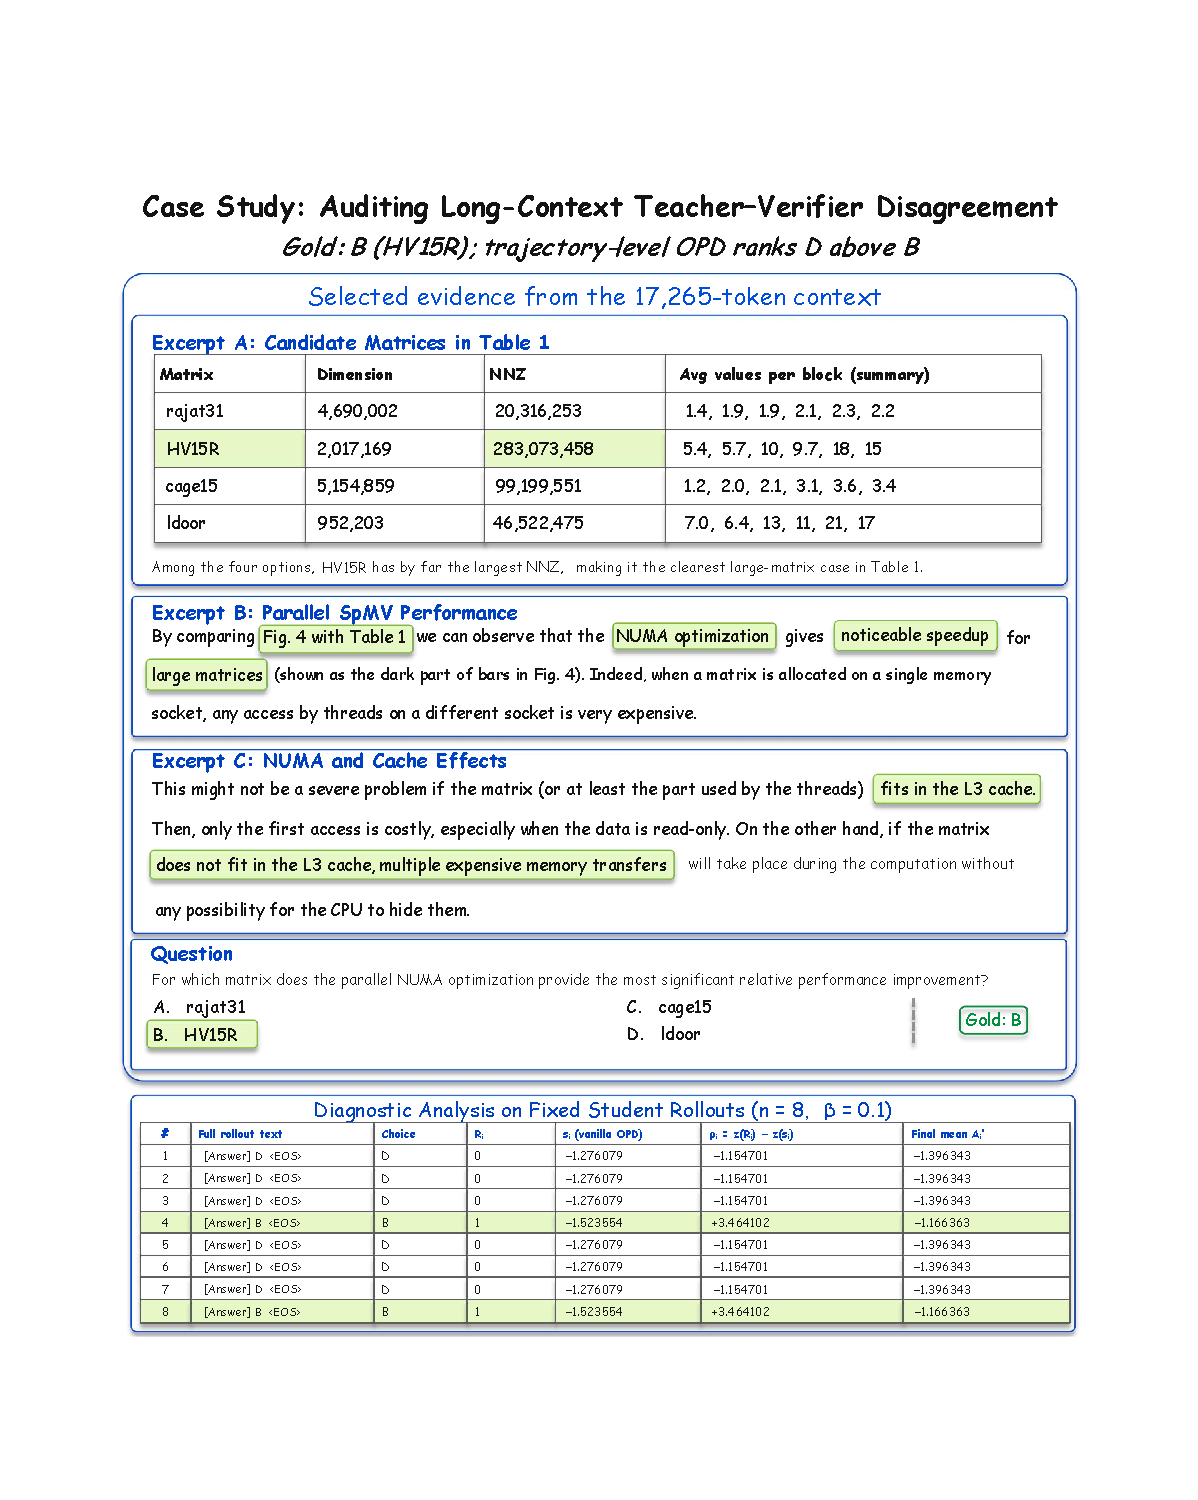
\includegraphics[width=1.08\textwidth]{Figures/gcopd_case_study/gcopd_long_context_case_study.pdf}%
}
\else
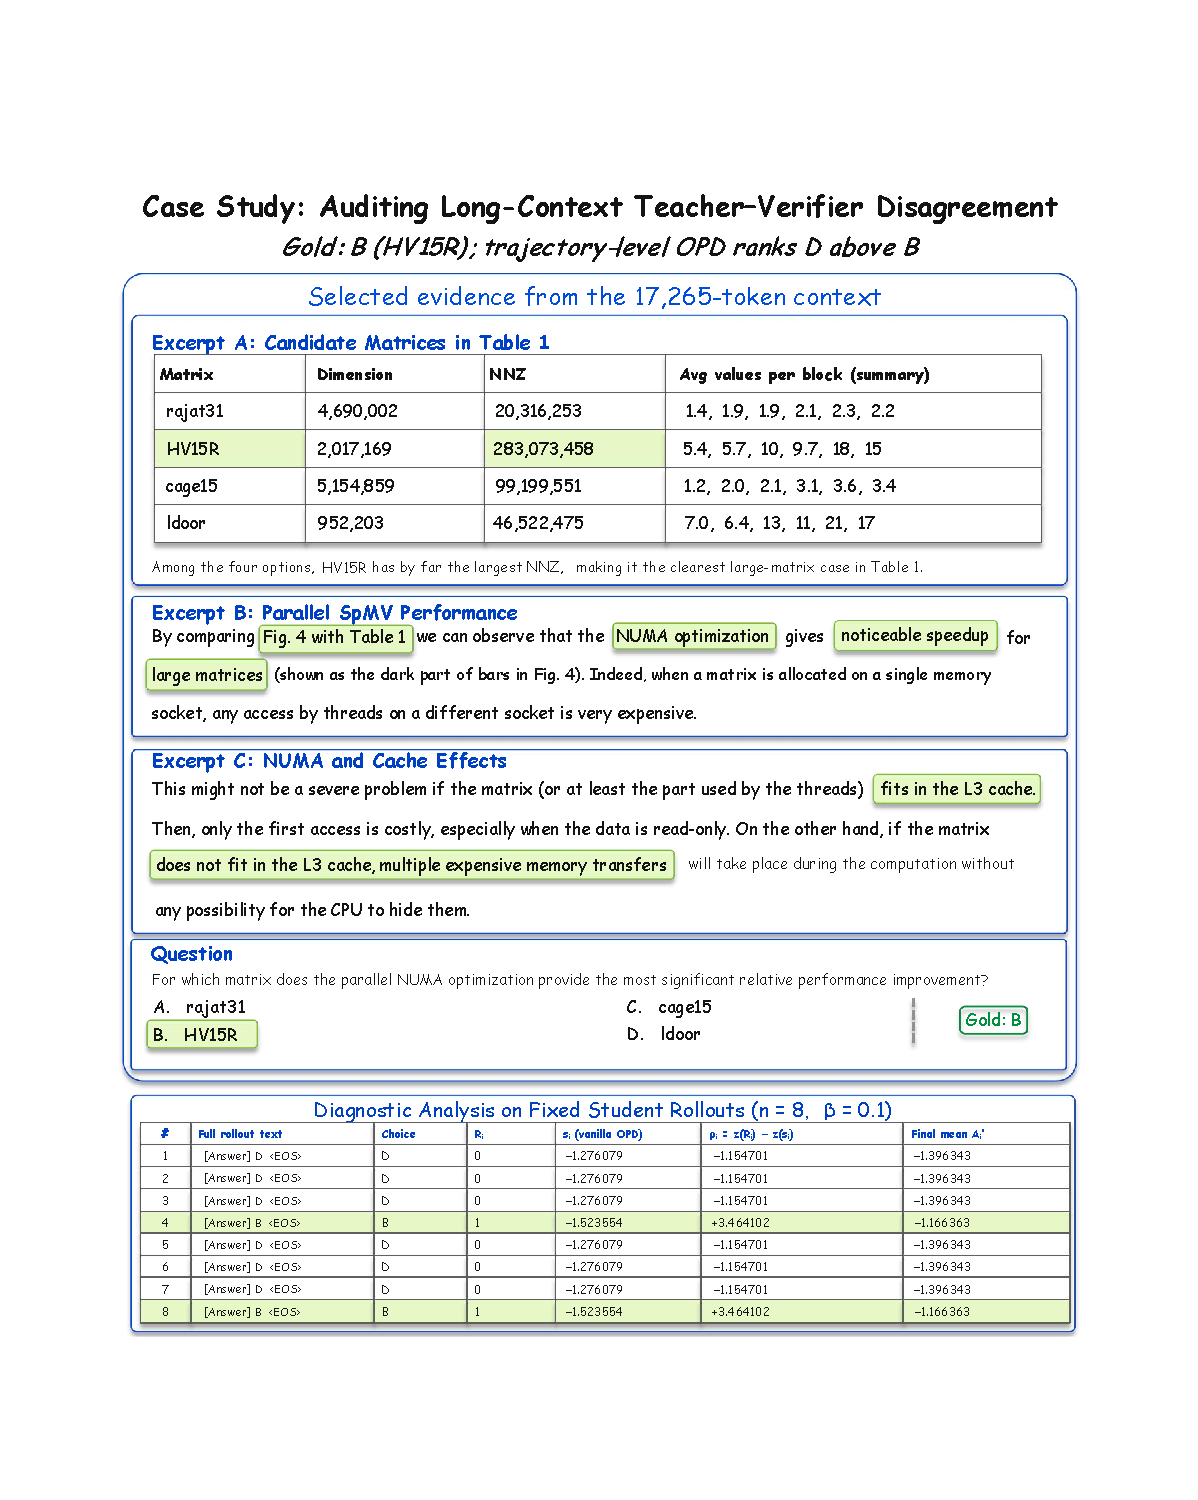
\includegraphics[width=0.96\textwidth]{Figures/gcopd_case_study/gcopd_long_context_case_study.pdf}
\fi
\caption{Illustrative fixed-rollout visualization for the 17,265-token case.
It reproduces the selected context evidence and all eight independently
rerolled student responses; the native label is B.}
\label{fig:case}
\ifdefined\GCOPDSingleColumnLayout
\end{figure}
\else
\end{figure*}
\fi

\ifdefined\GCOPDSingleColumnLayout
\begin{table}[H]
\else
\begin{table*}[!t]
\fi
\caption{Representative token-level RACA recalculations for the correct-B and
incorrect-D responses in Figure~\ref{fig:case} under the final GC-OPD setting.
Values are rounded; ranking checks use unrounded values.}
\label{tab:case-tokens}
\centering
{\small
\setlength{\tabcolsep}{2.15pt}
\resizebox{0.96\textwidth}{!}{%
\begin{tabular}{@{}lrrrrr@{\hspace{18pt}}lrrrrr@{}}
\toprule
\multicolumn{6}{c}{\textbf{Correct B response}, $\rho_{\mathrm{B}}=+3.464102$} &
\multicolumn{6}{c}{\textbf{Incorrect D response}, $\rho_{\mathrm{D}}=-1.154701$} \\
\cmidrule(lr){1-6}\cmidrule(lr){7-12}
Token & $A_t$ & $u_t$ & $c_t$ & $\Delta A_t$ & $\widehat A_t$ &
Token & $A_t$ & $u_t$ & $c_t$ & $\Delta A_t$ & $\widehat A_t$ \\
\midrule
\texttt{[} & -4.88599 & -1.85923 & 0.26959 & 0.09339 & -4.79260 &
\texttt{[} & -4.88599 & -1.98073 & 0.24248 & -0.02800 & -4.91399 \\
\texttt{Answer} & -0.02188 & 0.83034 & 1.39285 & 0.48250 & 0.46062 &
\texttt{Answer} & -0.02188 & 0.68817 & 1.33112 & -0.15370 & -0.17558 \\
\texttt{]} & -0.64095 & 0.48803 & 1.23928 & 0.42930 & -0.21165 &
\texttt{]} & -0.64095 & 0.34849 & 1.17250 & -0.13539 & -0.77634 \\
\texttt{B} & -1.91057 & -0.21400 & 0.89341 & 0.30949 & -1.60108 &
\texttt{D} & -0.66057 & 0.33773 & 1.16728 & -0.13479 & -0.79535 \\
\texttt{EOS} & -0.15839 & 0.75486 & 1.36047 & 0.47128 & 0.31290 &
\texttt{EOS} & -0.17101 & 0.60634 & 1.29421 & -0.14944 & -0.32046 \\
\bottomrule
\end{tabular}%
}
}
\ifdefined\GCOPDSingleColumnLayout
\end{table}
\else
\end{table*}
\fi
